\documentclass[11pt,letterpaper, leqno]{article}
\usepackage{latexsym}
\usepackage{amsmath}
\usepackage{amssymb}
\usepackage{amsthm}
\usepackage{float}
\usepackage{wrapfig}
\usepackage[caption = false]{subfig}
\topmargin -0.25in
\textheight 8.5in
\oddsidemargin 0.0in
\textwidth 6.5in

\RequirePackage{amsthm,amsmath,amsfonts,amssymb}
%\RequirePackage[numbers]{natbib}
\RequirePackage[authoryear]{natbib}%% uncomment this for author-year citations
\RequirePackage[colorlinks,citecolor=blue,urlcolor=blue]{hyperref}%% uncomment this for coloring bibliography citations and linked URLs
\RequirePackage{graphicx}%% uncomment this for including figures

\usepackage{tikz}
\usepackage{graphicx}
\usepackage{natbib}
\usepackage{authblk}
\usepackage[english]{babel}
\bibliographystyle{abbrvnat}
\setcitestyle{authoryear,open={(},close={)}}

% For the algorithm table
\usepackage{algorithm,algcompatible,amsmath}
\DeclareMathOperator*{\argmax}{\arg\!\max}
\DeclareMathOperator*{\argmin}{\arg\!\min}
% https://tex.stackexchange.com/q/83169/5764
\algnewcommand\INPUT{\item[\textbf{Input:}]}%
\algnewcommand\OUTPUT{\item[\textbf{Output:}]}%
%

% the settings of tikz is used for the optimization of the graphs  
\usetikzlibrary{shapes, arrows, calc, arrows.meta, fit, positioning} % these are the parameters passed to the library to create the node graphs  
\tikzset{  
    -Latex,auto,node distance =1.5 cm and 1.3 cm, thick,% node distance is the distance between one node to other, where 1.5cm is the length of the edge between the nodes  
    state/.style ={ellipse, draw, minimum width = 0.9 cm}, % the minimum width is the width of the ellipse, which is the size of the shape of vertex in the node graph  
    point/.style = {circle, draw, inner sep=0.18cm, fill, node contents={}},  
    bidirected/.style={Latex-Latex,dashed}, % it is the edge having two directions  
    el/.style = {inner sep=2.5pt, align=right, sloped}  
}  


\newtheorem{theorem}{Theorem}
\newtheorem{acknowledgement}[theorem]{Acknowledgement}
%\newtheorem{algorithm}[theorem]{Algorithm}
\newtheorem{axiom}[theorem]{Axiom}
\newtheorem{problem}[theorem]{Problem}
\newtheorem{remark}{Remark}
\newtheorem{claim}[theorem]{Claim}
\newtheorem{conclusion}[theorem]{Conclusion}
\newtheorem{condition}[theorem]{Condition}
\newtheorem{conjecture}[theorem]{Conjecture}
\newtheorem{corollary}{Corollary}
\newtheorem{criterion}[theorem]{Criterion}
\newtheorem{definition}{Definition}
\newtheorem{example}{Example}
\newtheorem{exercise}[theorem]{Exercise}
\newtheorem{lemma}{Lemma}
\newtheorem{proposition}{Proposition}
\newtheorem{thm}{Theorem}[section]
\newtheorem{lem}{Lemma}[section]
\newtheorem{prop}{Proposition}[section]
\newtheorem{defn}{Definition}[section]
\newtheorem{ex}{Example}[section]
\newtheorem{cor}{Corollary}[section]
\newtheorem{rem}{Remark}[section]
\newtheorem{rems}{Remarks}[section]
\numberwithin{equation}{section} 
\numberwithin{theorem}{section}
\numberwithin{lemma}{section} 
\numberwithin{corollary}{section}
\numberwithin{definition}{section}
\numberwithin{proposition}{section} 
\numberwithin{remark}{section}
\numberwithin{example}{section}
\newtheorem{assumption}{Assumption}
\DeclareMathOperator\supp{supp}

%\newcommand{\ex}{{\bf\sf E}}            %% expectation
\newcommand{\bfp}{{\bf P}}
\newcommand{\bfr}{{\bf R}}
\newcommand{\Var}{{\rm Var}}            %% 
\newcommand{\Cov}{{\rm Cov}}            %% 
\newcommand{\calc}{{\cal C}}            %%
\newcommand{\cald}{{\cal D}} 
\newcommand{\calf}{{\cal F}}            %%
\newcommand{\call}{{\cal L}}            
\newcommand{\al}{\alpha}                %%
\newcommand{\bt}{\beta}                %%
\newcommand{\ga}{\gamma}                %% abbreviated
\newcommand{\dt}{\delta}                %% greek letters
\newcommand{\la}{\lambda}               %%
\newcommand{\ep}{\epsilon}              %%
\newcommand{\sig}{\sigma}               %%
\newcommand{\tri}{\triangle}
\newcommand{\om}{\omega}                %%
\newcommand{\ra}{\rightarrow}           %%
\newcommand{\lra}{\longrightarrow}
\newcommand{\Ra}{\Rightarrow}           %% arrows
\newcommand{\subs}{\subseteq}           %% subset or equal to
\newcommand{\eqdef}{\stackrel{\triangle}{=}}
\newcommand{\hY}{\hat{Y}}
\newcommand{\hp}{\hat{p}}
\newcommand{\hX}{\hat{X}}
\newcommand{\hy}{\hat{y}}
\newcommand{\hQ}{\hat{Q}}
\newcommand{\Zh}{\hat{Z}}
\newcommand{\hla}{\hat{\lambda}}
\newcommand{\starti}{\parindent0pt\it}  %% start an italic line
\newcommand{\startb}{\parindent0pt\bf}  %% start a boldface line
\newcommand{\tril}{\triangle^-}
\newcommand{\trir}{\triangle^+}
\newcommand{\trilr}{\triangle^{\pm}}
\newcommand{\realR}{{{\rm I}\;\!\!\!{\rm R}}}
\newcommand{\probP}{{{\rm I}\;\!\!\!{\rm P}}}
\newcommand{\filtF}{{{\rm I}\;\!\!\!{\rm F}}}
\newcommand{\expeE}{{{\rm I}\;\!\!\!{\rm E}}}
\newcommand{\noin}{{\noindent}}
\newcommand{\doty}{{\dot{y}}}
\newcommand{\doth}{{\dot{h}}}
\newcommand{\dotx}{{\dot{x}}}
\newcommand{\dotu}{{\dot{u}}}
\newcommand{\dotf}{{\dot{f}}}
\newcommand{\dotg}{{\dot{g}}}
\newcommand{\ddoty}{{\ddot{y}}}
\newcommand{\ddoth}{{\ddot{h}}}
\newcommand{\ddotx}{{\ddot{x}}}
\newcommand{\ddotf}{{\ddot{f}}}
%\newcommand{\Var}{{\mbox{Var}}}
%\newcommand{\Cov}{{\mbox{Cov}}}
\newcommand{\T}{\intercal}

\newcommand{\ans}[1]{\boxed{\text{#1}}}
\newcommand{\vecs}[1]{\langle #1\rangle}
\renewcommand{\hat}[1]{\widehat{#1}}
\newcommand{\F}[1]{\mathcal{F}(#1)}
\renewcommand{\P}{\mathbb{P}}
\newcommand{\R}{\mathbb{R}}
\newcommand{\E}{\mathbb{E}}
\newcommand{\Z}{\mathbb{Z}}
\newcommand{\ind}{\mathbbm{1}}
\renewcommand{\qed}{\quad \blacksquare}
\newcommand{\brak}[1]{\left\langle #1 \right\rangle}
\newcommand{\bra}[1]{\left\langle #1 \right\vert}
\newcommand{\ket}[1]{\left\vert #1 \right\rangle}
\newcommand{\abs}[1]{\left\vert #1 \right\vert}

\usepackage{fancyhdr}
\pagestyle{fancy}
\lhead{ }
\rhead{\footnotesize{HW 9, APMA 1690 (Brown University)}}
\cfoot{\thepage}

\begin{document}
\begin{center}
{\bf \Large APMA1690: ~~Homework \# 9 ~~~(Due by 11pm on November 30)}
\end{center}

\medskip

\begin{center}
    ``\textit{He was too simple to wonder when he had attained humility. But he knew he had attained it, and he knew it was not disgraceful and it carried no loss of true pride.}"
\end{center}
\begin{flushright}
--- sentences from \textit{The Old Man and the Sea}, by Ernest Hemingway
\end{flushright}

\section{Review}

I would suggest you go through the review section before going to the problem set.

\subsection{Some Concepts in Graph Theory}

We list as follows the concepts needed for graphical models
\begin{itemize}
    \item A \textbf{graph} is an ordered pair $G=(V,E)$ comprising:
    \begin{itemize}
        \item $V$ is a set of \textbf{vertices}; the elements of $V$ are usually indexed by positive integers.
        \item $E$ is a subset of $\{(i,j) \,\vert\, i,j\in V \mbox{ and }i\ne j\}$, i.e., pairs of vertices; if we view the pairs as unordered, i.e., $(i,j)=(j,i)$ for all $i$ and $j$, this graph is called an \textbf{undirected graph}, otherwise, it is called a \textbf{directed graph}. (We focus on undirected graphs when talking about graphical models, i.e., we will keep assuming $(i,j)=(j,i)$.) 
    \end{itemize}
    
    \item For a given graph $G=(V,E)$, two vertices $i$ and $j$ are called \textbf{adjacent} if there is an edge between them, i.e., $(i,j)=(j,i)\in E$.
    
    \item For a given graph $G=(V,E)$ and a vertex $i\in V$, the \textbf{neighborhood} of $i$ is defined as the collection of vertices adjacent to $i$, i.e., $\mathcal{N}(i):=\{j\in V \,\vert\, (i,j)\in E\}$. Since we do not allow `self connecting edges' (i.e., vertices $i$ and $j$ should be different if then form an edge $(i,j)\in E$), we have $i\notin \mathcal{N}(i)$.
    
    \item For a given graph $G=(V,E)$, a set of vertices (i.e., a subset $c\subset V$) is called a \textbf{clique} if every pair of vertices in this set are adjacent. Furthermore, we denote $\mathcal{C}(G):=\{\mbox{all cliques of graph }G\,\}$. In addition, we adopt the convention that each vertex itself is a clique, i.e., $\{i\}\in\mathcal{C}(G)$ for all $i\in V$.
\end{itemize}
\begin{figure}[H]
    \centering
    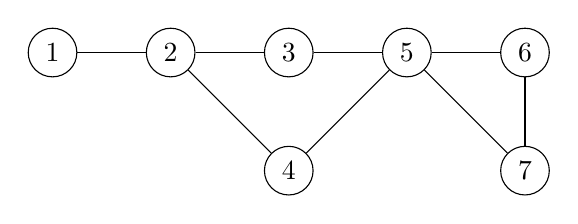
\begin{tikzpicture}[main/.style = {draw, circle}] 
\node[main] (1) {$1$}; 
\node[main] (2) [right of=1] {$2$};
\node[main] (3) [right of=2] {$3$};
\node[main] (4) [below of=3] {$4$};
\node[main] (5) [right of=3] {$5$};
\node[main] (6) [right of=5] {$6$};
\node[main] (7) [below of=6] {$7$};

\draw[-] (1) -- (2);
\draw[-] (2) -- (3);
\draw[-] (3) -- (5);
\draw[-] (2) -- (4);
\draw[-] (4) -- (5);
\draw[-] (5) -- (6);
\draw[-] (5) -- (7);
\draw[-] (6) -- (7);
\end{tikzpicture}
    \caption{A graph $G=(V,E)$ with $V=\{1,2,\ldots,7\}$\\ and $E=\{(1,2), (2,3), (2,4), (3,5), (4,5), (5,6), (5,7), (6,7)\}$.}\label{fig: graph example}
\end{figure}

Figure \ref{fig: graph example} provides an example of a graph. In this graph, for example, vertices 1 and 2 are adjacent, vertices 2 and 3 are adjacent. Additionally, the neighborhood of vertex 5 is $\mathcal{N}(5)=\{3,4,6,7\}$. We list all the elemnts of $\mathcal{C}(G)$ as follows
\begin{align}\label{eq: cliques of the graph example}
    \begin{aligned}
    & \{1\}, \{2\}, \{3\}, \{4\}, \{5\}, \{6\}, \{7\}, \\
    & \{1,2\}, \{2,3\}, \{2,4\}, \{3,5\}, \{4,5\}, \{5,6\}, \{5,7\}, \{6,7\}, \\
    & \{5,6,7\}.
    \end{aligned}
\end{align}

\subsection{Notations}

We also adopt the following notations
\begin{itemize}
    \item Let $G=(V,E)$ be a graph with $V=\{1,2,\ldots,d\}$ and $\boldsymbol{x}=(x_1,x_2,\ldots,x_d)^\T$ a vector in the product space $\mathcal{X}=\mathcal{X}_1\times\cdots\mathcal{X}_d$.
    \item For any subset $c=\{i_1,\ldots,i_k\}\subseteq V$ with $i_1<i_2<\cdots<i_k$, we denote $x_c:=(x_{i_1}, x_{i_2}, \ldots, x_{i_k})^\T$ and $\mathcal{X}_c:=\mathcal{X}_{i_1}\times\cdots\times\mathcal{X}_{i_k}$. For example, let $V=\{1,\ldots,7\}$ and $c=\{1,3,5\}$, then $x_c=(x_1, x_3, x_5)^\T$ and $\mathcal{X}_c=\mathcal{X}_1\times\mathcal{X}_3\times\mathcal{X}_5$.
\end{itemize}

\subsection{Application of Gibbs Sampling to the 2-Dimensional Ising Model}

This subsection helps discover a classical result from \cite{onsager1944crystal}\footnote{Professor Onsager taught statistical mechanics at Brown University and did the research work important enough to gain him the unshared Nobel Prize in Chemistry in 1968. However, ``the Great Depression limited Brown's ability to support a faculty member who was only useful as a researcher and not a teacher; he was let go by Brown, being hired by Yale University" (see \href{https://en.wikipedia.org/wiki/Lars_Onsager}{Wikipedia}).} in a numerical way.

\subsubsection{Periodic Lattices}\label{Periodic Lattices}

\texttt{(This subsection on periodic lattices is only for HW 9 and will not be required for the final exam.)}

We use periodic lattices, following the convention in the standard literature on the Ising model. The periodic structure will make the coding part easier. Without the periodic structure, we would have to deal with the boundaries of nonperiodic lattices separately.

A 3-by-3 periodic lattice $\Lambda_3$ is presented in Figure \ref{fig: 3-by-3 lattice}. An $N$-by-$N$ periodic lattice $\Lambda_N$ with a generic size $N$ is defined in a similar way. Specifically, for the vertex in the $i$-th row and $j$-th column of an $N$-by-$N$ periodic lattice, its neighbors are the following four vertices\footnote{For integers $a$ and $b$, the notation `$a \equiv b \ \operatorname{mod}\ (N)$' denotes the following: $N$ is a divisor of $a-b$, i.e., there exists an integer $k$ (not necessarily positive) such that $a-b=kN$.}
\begin{itemize}
    \item the vertex in the $k$-th row and $l$-th column, where $k\in\{1,\ldots,N\}$ with $k-1 \equiv i-1 \ \operatorname{mod}\ (N)$ and $l\in\{1,\ldots,N\}$ with $l-1 \equiv j-2 \ \operatorname{mod}\ (N)$.
    \item the vertex in the $k$-th row and $l$-th column, where $k\in\{1,\ldots,N\}$ with $k-1 \equiv i-1\ \operatorname{mod}\ (N)$ and $l\in\{1,\ldots,N\}$ with $l-1 \equiv j \ \operatorname{mod}\ (N)$.
    \item the vertex in the $k$-th row and $l$-th column, where $k\in\{1,\ldots,N\}$ with $k-1 \equiv i \ \operatorname{mod}\ (N)$ and $l\in\{1,\ldots,N\}$ with $l-1 \equiv j-1 \ \operatorname{mod}\ (N)$.
    \item the vertex in the $k$-th row and $l$-th column, where $k\in\{1,\ldots,N\}$ with $k-1 \equiv i-2 \ \operatorname{mod}\ (N)$ and $l\in\{1,\ldots,N\}$ with $l-1 \equiv j-1 \ \operatorname{mod}\ (N)$.
\end{itemize}
Neighborhoods of 5 and 3 of the 3-by-3 periodic lattice $\Lambda_3$ (see Figure \ref{fig: 3-by-3 lattice}) are presented in Figures \ref{fig: lattice illustration for the Ising model} and \ref{fig: lattice illustration for the Ising model 2}, respectively. The two figures visually interpret the complicated \href{https://en.wikipedia.org/wiki/Modular_arithmetic}{modular arithmetic} notation `$\operatorname{mod}\ (N)$' above.

\begin{figure}[h]
    \centering
    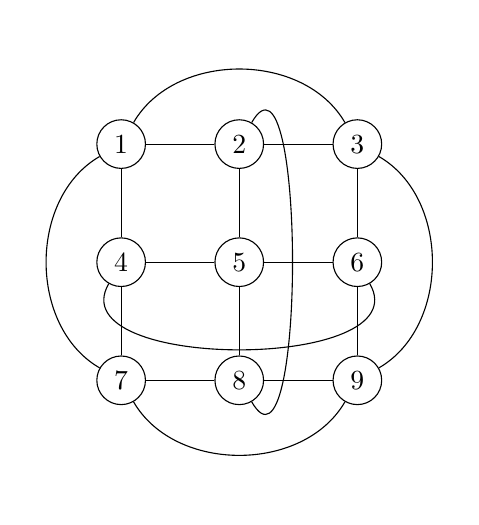
\begin{tikzpicture}[main/.style = {draw, circle}] 
\node[main] (1) {\textcolor{black}{$7$}}; 
\node[main] (2) [right of=1] {\textcolor{black}{$8$}};
\node[main] (3) [right of=2] {\textcolor{black}{$9$}};
\node[main] (4) [above of=1] {\textcolor{black}{$4$}};
\node[main] (5) [above of=2] {\textcolor{black}{$5$}};
\node[main] (6) [above of=3] {\textcolor{black}{$6$}};
\node[main] (7) [above of=4] {\textcolor{black}{$1$}};
\node[main] (8) [above of=5] {\textcolor{black}{$2$}};
\node[main] (9) [above of=6] {\textcolor{black}{$3$}};

\draw[-] (1) -- (2);
\draw[-] (2) -- (3);
\draw[-] (1) -- (4);
\draw[-] (2) -- (5);
\draw[-] (3) -- (6);
\draw[-] (4) -- (7);
\draw[-] (4) -- (5);
\draw[-] (5) -- (6);
\draw[-] (5) -- (8);
\draw[-] (6) -- (9);
\draw[-] (7) -- (8);
\draw[-] (8) -- (9);
\draw[-] (1) to [out=300,in=240] (3);
\draw[-] (2) to [out=300,in=60] (8);
\draw[-] (4) to [out=240,in=300] (6);
\draw[-] (7) to [out=60,in=120] (9);
\draw[-] (1) to [out=150,in=210] (7);
\draw[-] (3) to [out=30,in=330] (9);
\end{tikzpicture}
    \caption{A 3-by-3 periodic lattice $\Lambda_3$, which is a graph.}\label{fig: 3-by-3 lattice}
\end{figure}
\begin{figure}[h]
    \centering
    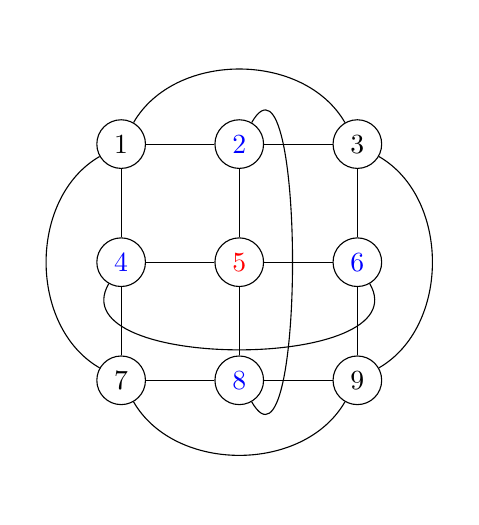
\begin{tikzpicture}[main/.style = {draw, circle}] 
\node[main] (1) {$7$}; 
\node[main] (2) [right of=1] {\textcolor{blue}{$8$}};
\node[main] (3) [right of=2] {$9$};
\node[main] (4) [above of=1] {\textcolor{blue}{$4$}};
\node[main] (5) [above of=2] {\textcolor{red}{$5$}};
\node[main] (6) [above of=3] {\textcolor{blue}{$6$}};
\node[main] (7) [above of=4] {$1$};
\node[main] (8) [above of=5] {\textcolor{blue}{$2$}};
\node[main] (9) [above of=6] {$3$};

\draw[-] (1) -- (2);
\draw[-] (2) -- (3);
\draw[-] (1) -- (4);
\draw[-] (2) -- (5);
\draw[-] (3) -- (6);
\draw[-] (4) -- (7);
\draw[-] (4) -- (5);
\draw[-] (5) -- (6);
\draw[-] (5) -- (8);
\draw[-] (6) -- (9);
\draw[-] (7) -- (8);
\draw[-] (8) -- (9);
\draw[-] (1) to [out=300,in=240] (3);
\draw[-] (2) to [out=300,in=60] (8);
\draw[-] (4) to [out=240,in=300] (6);
\draw[-] (7) to [out=60,in=120] (9);
\draw[-] (1) to [out=150,in=210] (7);
\draw[-] (3) to [out=30,in=330] (9);
\end{tikzpicture}
    \caption{The \textbf{neighborhood} of vertex $5$ (red) is $\mathcal{N}(5)=\{2,4,6,8\}$, presented in blue.}\label{fig: lattice illustration for the Ising model}
\end{figure}
\begin{figure}[h]
    \centering
    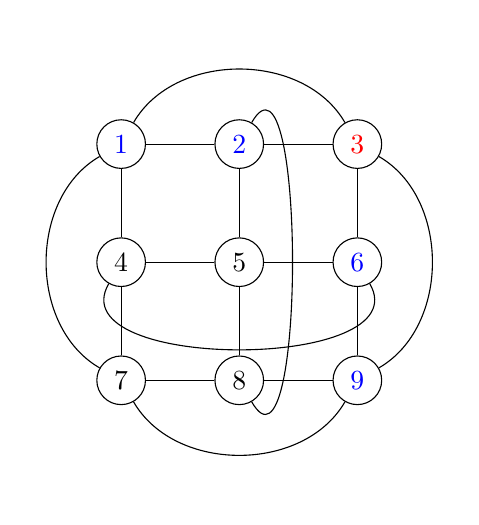
\begin{tikzpicture}[main/.style = {draw, circle}] 
\node[main] (1) {\textcolor{black}{$7$}}; 
\node[main] (2) [right of=1] {\textcolor{black}{$8$}};
\node[main] (3) [right of=2] {\textcolor{blue}{$9$}};
\node[main] (4) [above of=1] {\textcolor{black}{$4$}};
\node[main] (5) [above of=2] {\textcolor{black}{$5$}};
\node[main] (6) [above of=3] {\textcolor{blue}{$6$}};
\node[main] (7) [above of=4] {\textcolor{blue}{$1$}};
\node[main] (8) [above of=5] {\textcolor{blue}{$2$}};
\node[main] (9) [above of=6] {\textcolor{red}{$3$}};

\draw[-] (1) -- (2);
\draw[-] (2) -- (3);
\draw[-] (1) -- (4);
\draw[-] (2) -- (5);
\draw[-] (3) -- (6);
\draw[-] (4) -- (7);
\draw[-] (4) -- (5);
\draw[-] (5) -- (6);
\draw[-] (5) -- (8);
\draw[-] (6) -- (9);
\draw[-] (7) -- (8);
\draw[-] (8) -- (9);
\draw[-] (1) to [out=300,in=240] (3);
\draw[-] (2) to [out=300,in=60] (8);
\draw[-] (4) to [out=240,in=300] (6);
\draw[-] (7) to [out=60,in=120] (9);
\draw[-] (1) to [out=150,in=210] (7);
\draw[-] (3) to [out=30,in=330] (9);
\end{tikzpicture}
    \caption{The \textbf{neighborhood} of vertex $3$ (red) is $\mathcal{N}(3)=\{2,1,6,9\}$, presented in blue.}\label{fig: lattice illustration for the Ising model 2}
\end{figure}


\subsubsection{Ising Model PMF}

Suppose $\Lambda_N$ is an $N$-by-$N$ periodic lattice. Each vertex (also called a `site,' i.e., Section 18.3 of \cite{klenke2013probability}) is labeled by a positive integer, e.g., vertices of a 3-by-3 periodic lattice (see Figure \ref{fig: 3-by-3 lattice}) are labeled by $\{1,2,\ldots,9\}$.

At each vertex $k\in\Lambda_N$, there exists an atom with spin $s_k\in\{-1,1\}$. A \textbf{spin configuration} $\boldsymbol{s}$ is a vector of spin values assigned to the $N^2$ vertices, i.e.,
\begin{align*}
    \boldsymbol{s}=(s_k)_{k\in\Lambda} = \left( s_1, s_2, \ldots,s_{N^2} \right).
\end{align*}
Let $\mathcal{X}$ denote the collection of all possible spin configurations $\boldsymbol{s}$, i.e., 
\begin{align}\label{eq: definition of the state space}
    \mathcal{X}=\underbrace{\{-1,1\} \times \{-1,1\} \times \cdots \times \{-1,1\} }_{\mbox{\href{https://en.wikipedia.org/wiki/Cartesian_product}{Cartesian product} of $N^2$ sets}}.
\end{align}
It is straightforward that $\#\mathcal{X}=2^{N^2}$.

Because of the perturbation from heat, the spin values are not deterministic, i.e, $\boldsymbol{s}$ is a random vector. The Ising model gives PMFs describing the randomness of $\boldsymbol{s}$. A simplified Ising model-based PMF is the following one characterizing a ``\href{https://en.wikipedia.org/wiki/Ferromagnetism}{ferromagnetic} zero-field" model\footnote{The PMF $\pi_{N,\beta}(\boldsymbol{s}) =\frac{1}{Z_\beta}\cdot\exp\left\{-\beta\cdot\sum_{\langle i,j\rangle}s_is_j\right\}$ with an extra negative sign represents an ``\href{https://en.wikipedia.org/wiki/Antiferromagnetism}{antiferromagnetic} zero-field'' model, which is not of interest. }
\begin{align}\label{eq: Simplified Ising model}
    \begin{aligned}
        \pi_{N,\beta}(\boldsymbol{s}) &=\frac{1}{Z_\beta}\cdot\exp\left\{\beta\cdot\sum_{\langle i,j\rangle}s_is_j\right\} \\
    &= \frac{1}{Z_\beta}\cdot\exp\left\{\beta\cdot \left( \sum_{\text{all edges }(i,j) \text{ on the $N$-by-$N$ periodic lattice}} s_is_j \right)\right\},
    \end{aligned}
\end{align}
where $\langle i,j \rangle$ denotes that $i$ and $j$ are neighbors. The PMF formula in Eq.~\eqref{eq: Simplified Ising model} is called the 2-dimensional Ising model\footnote{German pronunciation is like the English word ``easing" (see the remark in Example 18.16 of \cite{klenke2013probability}).}. The notations above are explained as follows:
\begin{itemize}
\item $\sum_{\langle i,j\rangle}$ denotes the sum over all pairs $(i,j)$ such that $i$ and $j$ are neighbors.  It is the standard notation in the Ising model literature, e.g., the Wikipedia page on the \href{https://en.wikipedia.org/wiki/Ising_model}{Ising Model}. 
    
\item $\beta$ is a model parameter. Specifically, $\beta=1/T$, where $T$ indicates the temperature of the magnetic system.

\item $Z_\beta=\sum_{\boldsymbol{s}\in\mathcal{X}}\exp\left\{ \beta\cdot\sum_{\langle i,j\rangle}s_is_j\right\}$ is the normalizing constant. As a function of $\beta$, the quantity $Z_\beta$ is the \href{https://en.wikipedia.org/wiki/Partition_function_(statistical_mechanics)}{partition function} of the model. The letter Z stands for the German word \textit{Zustandssumme}, ``sum over states," and $\sum_{\boldsymbol{s}\in\mathcal{X}}$ is the sum over all possible spin configurations.

\item $H_N(\boldsymbol{s}) = - \sum_{\langle i,j\rangle} s_i s_j$ presents the energy of the magnetic system, and $\pi_{N,\beta}(\boldsymbol{s}) =\frac{1}{Z_\beta}\cdot\exp\left\{ - \beta\cdot H_N(\boldsymbol{s}) \right\}$ is referred to as the \href{https://en.wikipedia.org/wiki/Boltzmann_distribution}{Boltzmann distribution} of the magnetic system in the statistical mechanics literature. Notably, the negative sign in $H_N(\boldsymbol{s})$ and the negative sign in the Boltzmann distribution are canceled out. Forgetting to cancel out the negative sign will make a ferromagnetic model become an antiferromagnetic model.
\end{itemize}

\subsubsection{Curie Temperature}\label{Curie Temperature}


The \href{https://en.wikipedia.org/wiki/Curie_temperature}{Curie temperature} is the one above which certain materials lose their permanent magnetic properties. The Curie temperature is named after \href{https://en.wikipedia.org/wiki/Pierre_Curie}{Pierre Curie}. In this section, we describe the Curie temperature using the Ising model. The discussion in this section provides a nontrivial question that can be solved by the Gibbs sampling algorithm.

Suppose the distribution $\pi_{N,\beta}(\boldsymbol{s})$ of spin configurations $\boldsymbol{s}$ is given by the ferromagnetic zero-field model in Eq.~\eqref{eq: Simplified Ising model}. Macroscopically, the individual spins cannot be observed, but the following average magnetization can
\begin{align}\label{eq: average magnetization}
    m_N(\beta):=\sum_{\boldsymbol{s}\in \mathcal{X}} \pi_{N,\beta}(\boldsymbol{s}) \cdot \left\vert\frac{\sum_{i\in\Lambda_N}s_i}{N^2}\right\vert=\mathbb{E}_{\pi_{N,\beta}}\left\vert\frac{\sum_{i\in\Lambda_N}s_i}{N^2}\right\vert,
\end{align}
where ``$\sum_{\boldsymbol{s}\in \mathcal{X}}$" means the sum over all possible spin configurations. If we consider a very large system, then we are close to the so-called \href{https://en.wikipedia.org/wiki/Thermodynamic_limit}{thermodynamic limit}
\begin{align}\label{eq: def thermodynamic limit}
    m(\beta):=\lim_{N\rightarrow\infty}m_N(\beta).
\end{align}
The interpretation of $m(\beta)$ is roughly presented as follows: when $m(\beta)>0$, the material of interest is magnetic; when $m(\beta)=0$, it is not magnetic. The magic of Curie Temperature comes from this limiting procedure in Eq.~\eqref{eq: def thermodynamic limit}. \cite{peierls1936ising} essentially showed that there exists a critical value $\beta_C=\frac{1}{T_C}$, where $T_C$ is the Curie temperature of interest, such that 
\begin{align}\label{eq: def of beta C}
    m(\beta)\left\{
    \begin{aligned}
    >0,\ \ \mbox{ if }\beta>\beta_C,\\
    =0,\ \ \mbox{ if }\beta<\beta_C.
    \end{aligned}
    \right.
\end{align}
That is, we have the Curie temperature $T_C$ is represented as follows
\begin{align}\label{eq: representation of Curie temperature}
    T_C=\frac{1}{\beta_C}.
\end{align}
Below the Curie temperature, the material of interest is magnetic; above the Curie temperature, it is not. \cite{onsager1944crystal} provided the exactly value of $\beta_C$ as follows
\begin{align}\label{eq: beta C}
    \boxed{\beta_C=\frac{\log(1+\sqrt{2})}{2} \approx0.44.}
\end{align}


\subsubsection{Estimation of $\beta_C$}

Mathematically deriving the value $\beta_C$ in Eq.~\eqref{eq: beta C} is nearly a Nobel prize-level question. Using the Gibbs sampling, we can estimate this value numerically. To estimate $\beta_C$, we need to estimate the $m(\beta)$ defined in Eq.~\eqref{eq: def thermodynamic limit}. When the size $N$ of the periodic lattice $\Lambda_N$ is large, we have $m(\beta)\approx m_N(\beta)$.

Suppose we have a homogeneous Markov chain (HMC) 
\begin{align}\label{eq: such a MC}
    \left\{ \boldsymbol{X}^{(n)}=\left( X_1^{(n)}, X_2^{(n)},\ldots, X_{N^2}^{(n)} \right) \right\}_{n=0}^\infty
\end{align}
whose state space is the $\mathcal{X}$ defined in Eq.~\eqref{eq: definition of the state space}; furthermore, this HMC is irreducible and apperiodic, and its stationary distribution is the $\pi_{N,\beta}(\boldsymbol{s})$ defined in Eq.~\eqref{eq: Simplified Ising model}. Visualizations of $\boldsymbol{X}^{(10000)}$ with lattice size $N=100$ for different $\beta$ values are presented in Figure \ref{fig: spin configurations for different temperatures}.

\begin{figure}
    \centering
    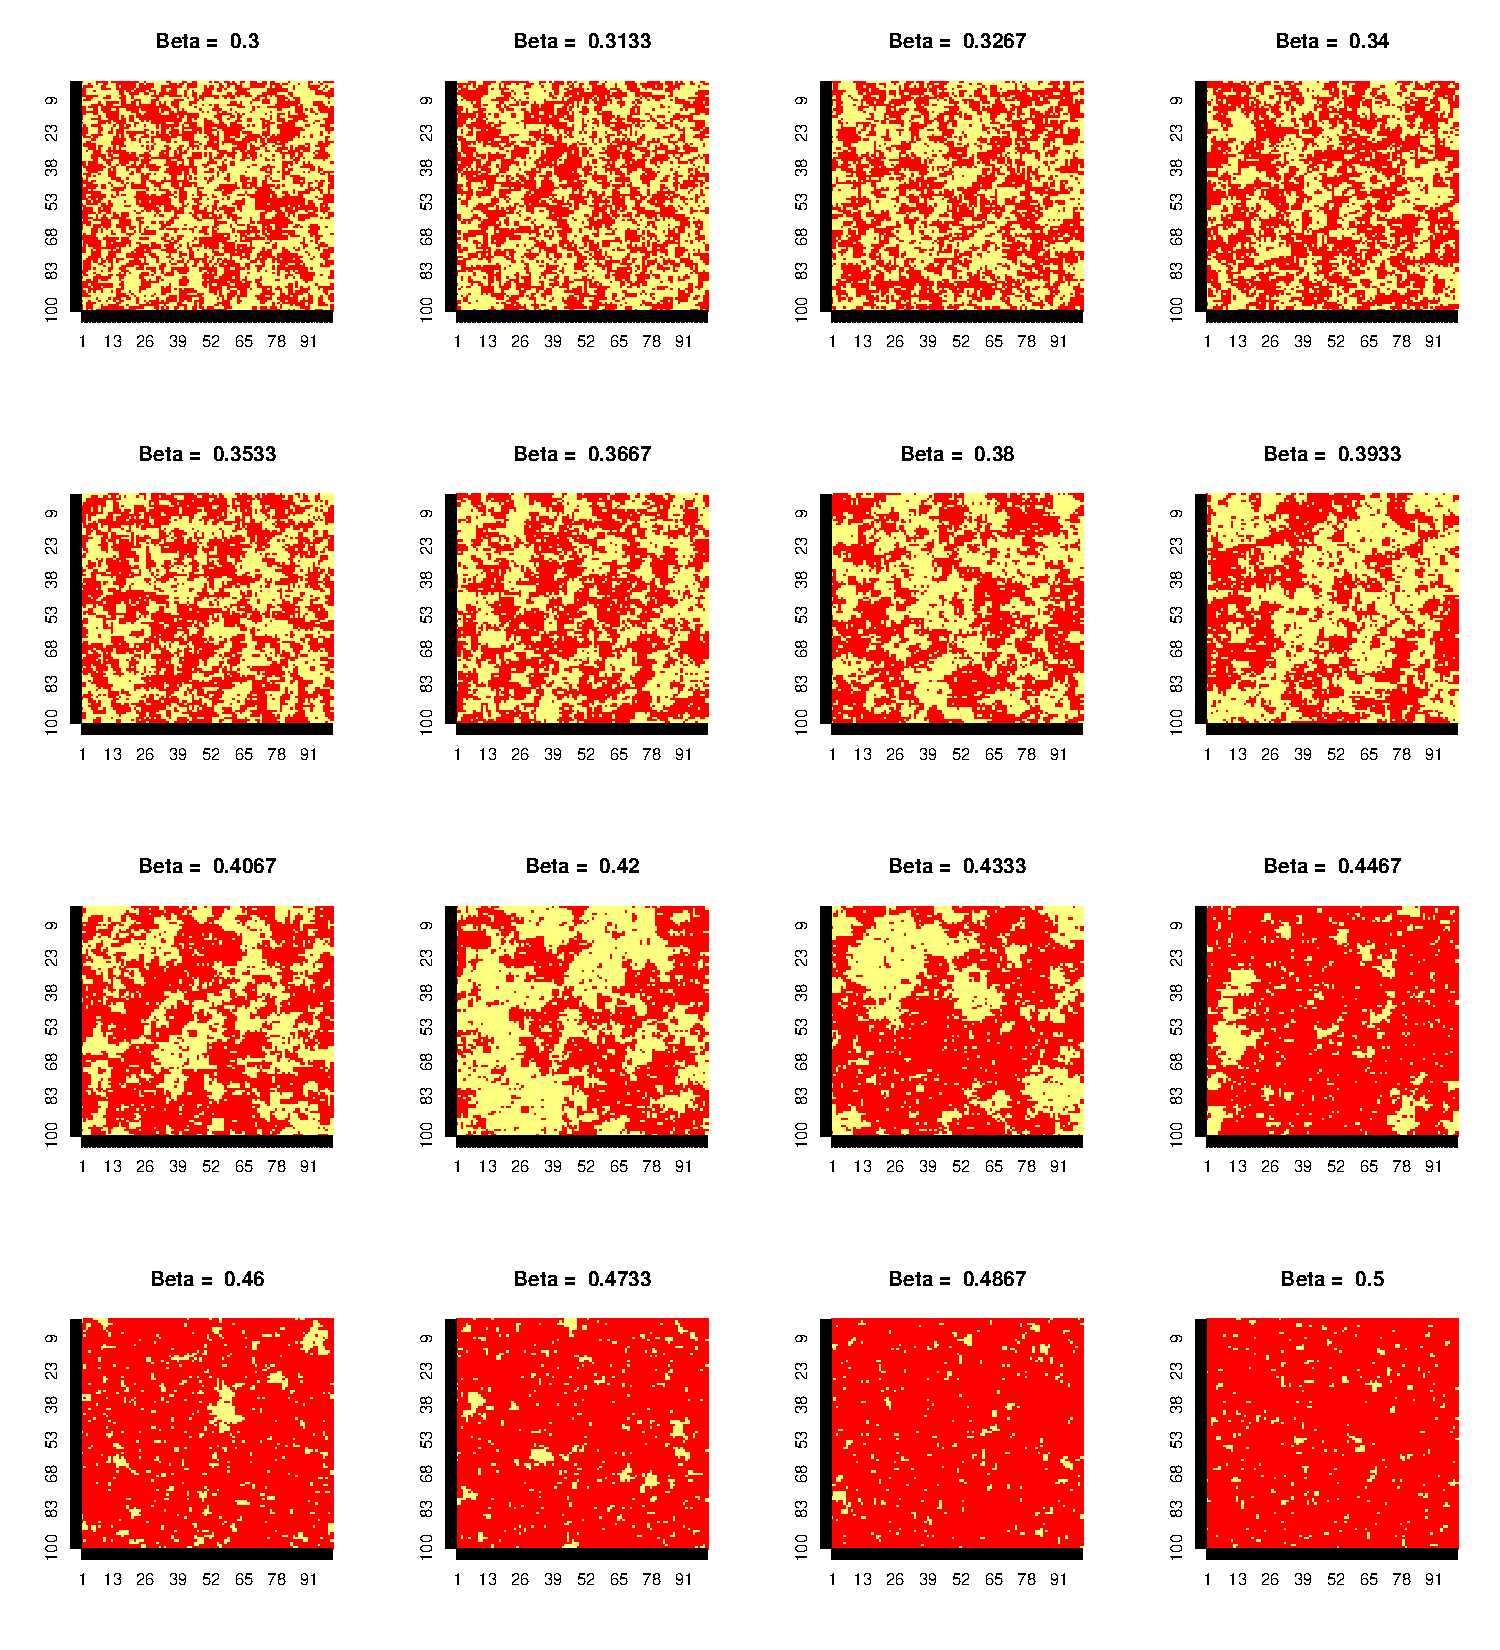
\includegraphics[scale=0.65]{Ising100_16by16.pdf}
    \caption{Visualizations of $\boldsymbol{X}^{(10000)}$ with lattice size $N=100$ for different $\beta$ values. Recall the critical value $\beta_C=\frac{\log(1+\sqrt{2})}{2} \approx0.44$.}
    \label{fig: spin configurations for different temperatures}
\end{figure}

Then, the ergodic theorem implies the following with probability one
\begin{align*}
    \lim_{n\rightarrow\infty} \left\{ \frac{1}{n}\sum_{i=1}^n \left\vert\frac{\sum_{k\in\Lambda_N} X^{(i)}_k}{N^2}\right\vert \right\} = m_N(\beta).
\end{align*}
Therefore, when both the lattice size $N$ and sample size $n$ are large, we have
\begin{align}\label{eq: estimation of m beta}
    m(\beta)\approx m_N(\beta) \approx \frac{1}{n}\sum_{i=1}^n \left\vert\frac{\sum_{k\in\Lambda_N} X^{(i)}_k}{N^2}\right\vert =: \widehat{v}_{N,n}(\beta).
\end{align}
Then, we can apply Eq.~\eqref{eq: estimation of m beta} (i.e., the estimator $\widehat{v}_{N,n}(\beta)$) to estimate $m(\beta)$, which help us estimate $\beta_C$. Now, it remains to get such an HMC in Eq.~\eqref{eq: such a MC}, which can be done through the Gibbs sampling.

\subsubsection{Application of the Gibbs Sampling to Ising Model}

For each vertex $i$, we define the neighborhood $\mathcal{N}(i)$ of $i$ by the following
\begin{align*}
    \mathcal{N}(i)&:=\{\mbox{the neighbors of site }i\}.
\end{align*}

Suppose we are interested in the spin $s_{i^*}$ at the vertex $i^*$. The Boltzmann distribution $\pi_{N,\beta}(\boldsymbol{s})$ in Eq.~\eqref{eq: Simplified Ising model} can be represented as follows
\begin{align}\label{eq: Boltzmann distribution of Ising model for the graphical purpose}
    \pi_{N,\beta}(\boldsymbol{s}) = \frac{1}{Z_\beta}\cdot\exp\left\{\beta\left[\sum_{j\in\mathcal{N}(i^*)}s_{i^*}s_j\right]+\beta\left[\sum_{\langle i',j'\rangle\mbox{ and }i',j'\ne i^*}s_{i'}s_{j'}\right]\right\}.
\end{align}

\subsection{Conditional Distributions}

A key quantity in the Gibbs sampling (see Algorithm \ref{algorithm: Gibbs sampling}) is the conditional distribution of $s_{i^*}$ given the values of other coordinates, i.e.,
\begin{align*}
    \pi_{N,\beta}(s_{i^*}\vert\boldsymbol{s}_{-i^*})= \pi_{N,\beta}(s_{i^*}\vert s_1,\ldots,s_{i^*-1},\, s_{i^*+1},\ldots,s_{N^2}).
\end{align*}
Using the representation in Eq.~\eqref{eq: Boltzmann distribution of Ising model for the graphical purpose}, the conditional distribution $\pi_{N,\beta}(s_{i^*}\vert\boldsymbol{s}_{-i^*})$ can be represented as follows
\begin{align}\label{eq: the important cancelation of the Ising model}
    \begin{aligned}
    \pi_{N,\beta}(s_{i^*}\vert\boldsymbol{s}_{-i^*}) &= \frac{\pi_{N,\beta}(\boldsymbol{s})}{\sum_{s_{i^*}\in\{-1,1\}}\pi_{N,\beta}(\boldsymbol{s})} \\
    &= \frac{\frac{1}{Z_\beta}\cdot\exp\left\{\beta\left[\sum_{\langle i',j'\rangle\mbox{ and }i',j'\ne i^*}s_{i'}s_{j'}\right]\right\}\cdot \textcolor{blue}{\exp\left\{\beta\left[\sum_{j\in\mathcal{N}(i^*)}s_{i^*}s_j\right]\right\}}}{\frac{1}{Z_\beta}\cdot\exp\left\{\beta\left[\sum_{\langle i',j'\rangle\mbox{ and }i',j'\ne i^*}s_{i'}s_{j'}\right]\right\}\cdot \textcolor{blue}{\sum_{s_{i^*}\in\{-1,1\}}\exp\left\{\beta\left[\sum_{j\in\mathcal{N}(i^*)}s_{i^*}s_j\right]\right\}}} \\
    &= \frac{\exp\left\{\beta\left[\sum_{j\in\mathcal{N}(i^*)}s_{i^*}s_j\right]\right\}}{\sum_{s_{i^*}\in\{-1,1\}}\exp\left\{\beta\left[\sum_{j\in\mathcal{N}(i^*)}s_{i^*}s_j\right]\right\}} \\
    &= \frac{\exp\left\{\beta\left[\sum_{j\in\mathcal{N}(i^*)}s_{i^*}s_j\right]\right\}}{\exp\left\{-\beta\left[\sum_{j\in\mathcal{N}(i^*)} s_j\right]\right\} + \exp\left\{\beta\left[\sum_{j\in\mathcal{N}(i^*)} s_j\right]\right\}},
    \end{aligned}
\end{align}
More precisely, we have the following
\begin{align}\label{eq: conditional distribition}
    \begin{aligned}
        & \pi_{N,\beta}(\, 1 \, \vert\boldsymbol{s}_{-i^*}) = \frac{\exp\left\{\beta\left[\sum_{j\in\mathcal{N}(i^*)} s_j\right]\right\}}{\exp\left\{-\beta\left[\sum_{j\in\mathcal{N}(i^*)} s_j\right]\right\} + \exp\left\{\beta\left[\sum_{j\in\mathcal{N}(i^*)} s_j\right]\right\}}, \\
    & \pi_{N,\beta}( \, -1 \, \vert\boldsymbol{s}_{-i^*}) = \frac{\exp\left\{-\beta\left[\sum_{j\in\mathcal{N}(i^*)} s_j\right]\right\}}{\exp\left\{-\beta\left[\sum_{j\in\mathcal{N}(i^*)} s_j\right]\right\} + \exp\left\{\beta\left[\sum_{j\in\mathcal{N}(i^*)} s_j\right]\right\}}.
    \end{aligned}
\end{align}
The factor $\frac{1}{Z_\beta}\cdot\exp\left\{\beta\left[\sum_{\langle i',j'\rangle\mbox{ and }i',j'\ne i^*}s_{i'}s_{j'}\right]\right\}$ in Eq.~\eqref{eq: the important cancelation of the Ising model} is canceled out. This cancelation is extremely important as it reduces the redundant computation.

\subsection{Sampling from Conditional Distributions}

To sample a random variable $X_{i^*}^{(n)}$ from the conditional distribution $\pi_{N,\beta}(\,\cdot\, \vert\boldsymbol{s}_{-i^*})$ defined in Eq.~\eqref{eq: conditional distribition}, we can adopt the following procedure:
\begin{itemize}
    \item Compute $a \leftarrow \exp\left\{\beta\left[\sum_{j\in\mathcal{N}(i^*)} s_j\right]\right\}$.
    
    \item Compute $b \leftarrow \exp\left\{-\beta\left[\sum_{j\in\mathcal{N}(i^*)} s_j\right]\right\}$.
    
    \item Compute $p\leftarrow \frac{a}{a+b}$.

    \item Generate $Z\sim \operatorname{Bernoulli}(p)$, i.e., $\mathbb{P}(Z=1)=p$ and $\mathbb{P}(Z=0)=1-p$.

    \item $X_{i^*}^{(n)} \leftarrow 2\cdot Z-1$, i.e., $\mathbb{P}(X_{i^*}^{(n)}=1) = \frac{a}{a+b}$ and $\mathbb{P}(X_{i^*}^{(n)}=-1) = \frac{b}{a+b}$.
\end{itemize}
With the procedure above, we can sample the HMC in Eq.~\eqref{eq: such a MC} through Gibbs sampling (Algorithm \ref{algorithm: Gibbs sampling}).

\subsubsection{Numerical Experiment}

As an ending section, we present a numerical experiment of the estimation $m(\beta) \approx \widehat{v}_{N,n}(\beta)$ presented in Eq.~\eqref{eq: estimation of m beta}. In this experiment, we choose the lattice size to be $N=100$ and the sample size to be $n=10000$. The `$\widehat{v}_{N,n}(\beta)$ vs. $\beta$' plot is presented in Figure \ref{fig: M_beta}, where the vertical dashed line indicates the critical value $\beta_C\approx 0.44$. Figure \ref{fig: M_beta} is compatible with Eq.~\eqref{eq: def of beta C}.

\begin{figure}
    \centering
    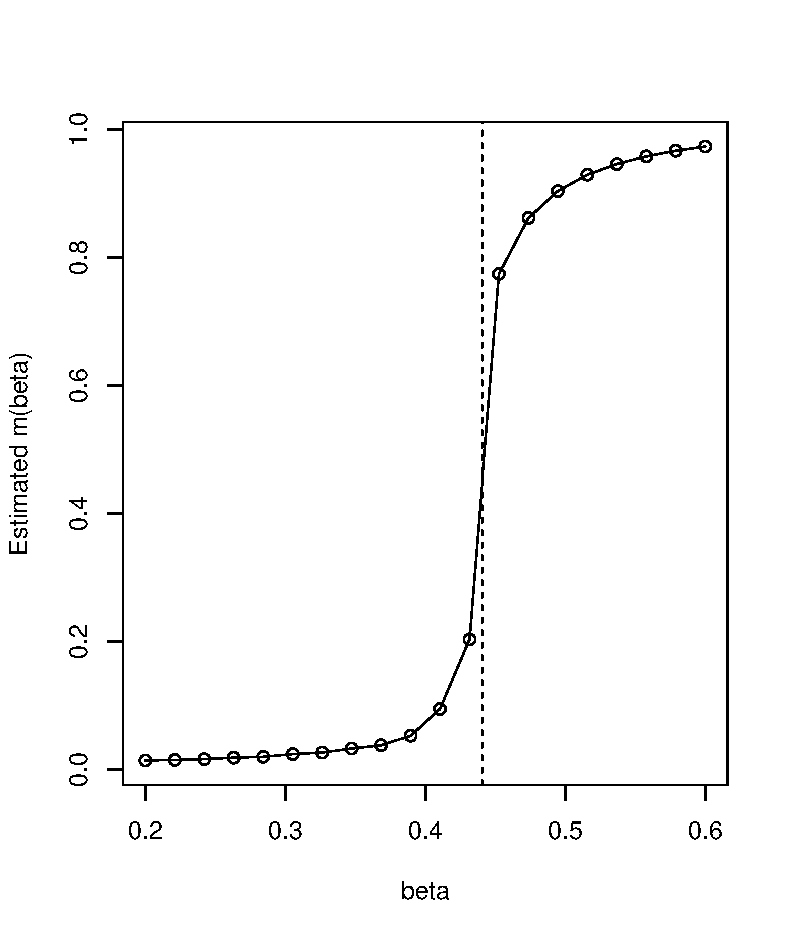
\includegraphics[scale=0.6]{M_beta.pdf}
    \caption{The `$\widehat{v}_{N,n}(\beta)$ vs. $\beta$' plot. The vertical dashed line indicates the critical value $\beta_C\approx 0.44$.}
    \label{fig: M_beta}
\end{figure}

\subsubsection{Appendix: Gibbs Sampling}

\begin{algorithm}[H]
\caption{: Gibbs Sampling}\label{algorithm: Gibbs sampling}
\begin{algorithmic}[1]
    \INPUT (i) the given distribution $\pi(\xi_1,\ldots,\xi_d)$; (ii) a starting point $\boldsymbol{x}^{(0)}=(\xi^{(0)}_1,\ldots, \xi^{(0)}_d)^\T$.
    \OUTPUT A homogeneous Markov chain $\{\boldsymbol{X}^{(n)}=(\xi_1^{(n)}, \ldots, \xi_d^{(n)})^\T\}_{n=0}^\infty$ with $\pi$ as its stationary distribution.
    \STATE Set $\boldsymbol{X}^{(0)}  \leftarrow\boldsymbol{x}^{(0)}$.
    \FORALL{$n=1,2,\ldots$,}
    \STATE Sample $\xi_1^{(n)}\sim \pi_{1\vert-1}(\xi_1\vert \xi_2^{\textcolor{blue}{(n-1)}}, \ldots, \xi_d^{\textcolor{blue}{(n-1)}})$
    \FORALL{$j=2,\ldots,d$}
    \STATE Sample $\xi_j^{(n)} \sim \pi_{j\vert-j}(\xi_j \vert \xi_1^{\textcolor{red}{(n)}},\ldots,\xi_{j-1}^{\textcolor{red}{(n)}}, \xi_{j+1}^{\textcolor{blue}{(n-1)}},\ldots, \xi_{d}^{\textcolor{blue}{(n-1)}})$
    \ENDFOR
    $\boldsymbol{X}^{(n)} \leftarrow (\xi_1^{(n)}, \xi_2^{(n)}, \ldots, \xi_d^{(n)})^\T$
    \ENDFOR
\end{algorithmic}
\end{algorithm}


\newpage

\section{Problem Set}

\begin{enumerate}

\item (3 points) Let $G=(V,E)$ be a graph. Prove the following identity
\begin{align}\label{eq: clique-nbh identity}
    \mathcal{N}(i)\bigcup\{i\}=\left(\bigcup_{c\in\mathcal{C}(G) \mbox{ and }i\in c} c\right),
\end{align}
where the union sign $\bigcup$ on the right hand side of Eq.~\eqref{eq: clique-nbh identity} denotes the union over all cliques $c$ such that $i\in c$. For the details of the union notation, please refer to the Wikipedia page on `\href{https://en.wikipedia.org/wiki/Union_(set_theory)}{Union (set theory)},' especially the ``arbitrary unions" section therein.

Hint: see the definition of cliques.

Remark: The set identity in Eq.~\eqref{eq: clique-nbh identity} partially implies the \href{https://en.wikipedia.org/wiki/Hammersley-Clifford_theorem}{Hammersley–Clifford theorem}.

    \color{blue}
        \begin{align*}
            \mathcal{N}(i) \cup \{i\} &= \{j \in V: (i, j) \in E\} \cup \{i\}\\
                &= \{i, j_1, \dots,\; j_k:\; (i, j_1), \dots, (i, j_k) \in E\}\\
                &= \{c \in \mathcal{C}(G): i \in c\}\\
                &= \bigcup_{\begin{subarray}{c}
                    c \in \mathcal{C}(G)\\
                    i \in c
                \end{subarray}} c\qed
        \end{align*}
    \color{black}
\pagebreak

\item (7 points) In this question, we consider the Ising model on a 100-by-100 \textbf{periodic} lattice (i.e., the lattice size $N=100$). We focus on the following 20 values of the parameter $\beta$
\begin{align}\label{eq: betas}
    \beta \in \left\{0.2 + 0.02k \,\vert\, k=1,2,\ldots,20\right\}.
\end{align}
Please do the following tasks using Gibbs sampling: 
\begin{itemize}
    \item For each of the $\beta$ values in Eq.~\eqref{eq: betas}, generate the sequence
\begin{align}\label{eq: finite sequence}
    \left\{ \boldsymbol{X}^{(i)}=\left( X_1^{(i)}, X_2^{(i)},\ldots, X_{N^2}^{(i)} \right) \right\}_{i=0}^{1000},
\end{align}
which is the first 1000 (or 1001) components of an irreducible and aperiodic HMC with the $\pi_{N,\beta}$ in Eq.~\eqref{eq: Simplified Ising model} as its stationary distribution.

\item Plot $\boldsymbol{X}^{(1000)}$ for $\beta\in\{0.32, 0.4, 0.44, 0.6\}$. Each of your four plots should be similar to one of the panels in Figure \ref{fig: spin configurations for different temperatures}.

\item For each of the twenty $\beta$ values in Eq.~\eqref{eq: betas}, compute 
\begin{align*}
    \widehat{v}(\beta):= \frac{1}{1000}\sum_{i=1}^{1000} \left\vert\frac{\sum_{k\in\Lambda_N} X^{(i)}_k}{N^2}\right\vert.
\end{align*}

\item List the following twenty values of $\widehat{v}(\beta)$
\begin{align}\label{eq: 20 v values}
    \left\{ \widehat{v}(\beta) \,\Big\vert\, \beta=0.2 + 0.02k \text{ for } k=1,2,\ldots,20\right\}.
\end{align}

\item Plot the twenty values in Eq.~\eqref{eq: 20 v values} in a `$\widehat{v}(\beta)$ vs. $\beta$' fashion, which should be similar to Figure \ref{fig: M_beta}.

\end{itemize}

Please provide your code for completing each of the tasks.
\end{enumerate}

\color{blue}
        Here are the plots for $\beta \in \{0.32, 0.4, 0.44, 0.6\}$:
        \begin{center}
            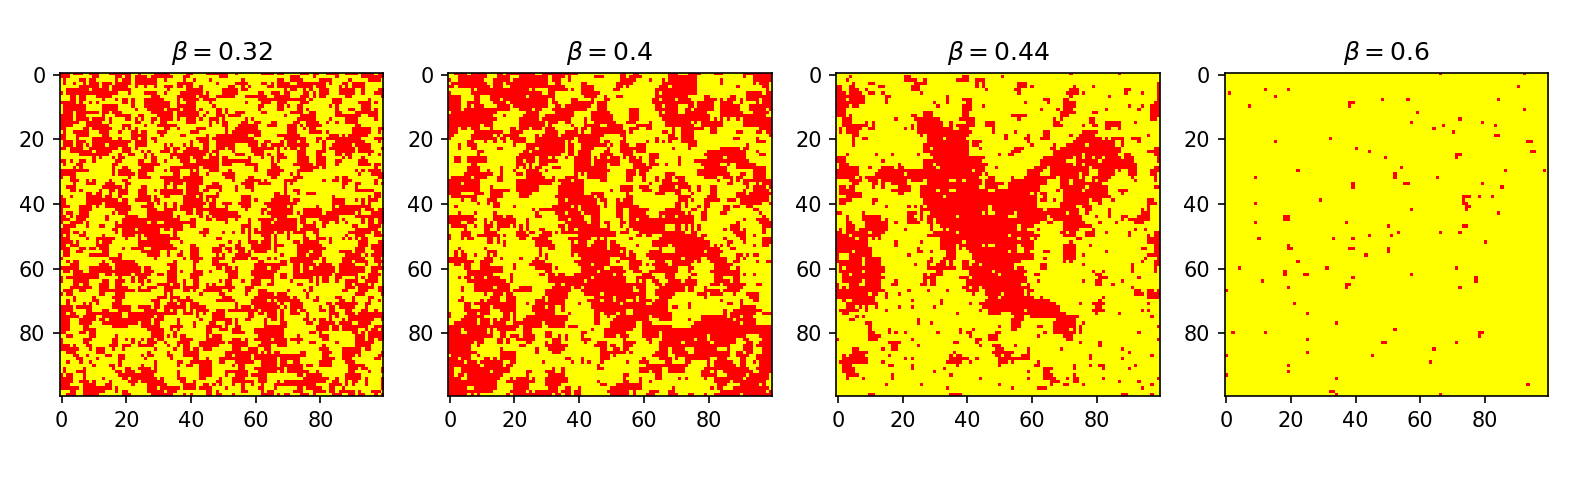
\includegraphics[width=\textwidth]{Images/X1000.png}
        \end{center}

        \pagebreak
        The full list of values for $\widehat{v}(\beta)$ along with the plot of $\hat v(\beta)$ vs. $\beta$ are below:

        \vspace*{0.1in}

        \begin{tabular*}{1in}{|c|c|} 
            \hline 
            $\beta$ & $\hat{v}(\beta)$\\ 
            \hline 
            0.22 & 0.0116\\ 
            0.24 & 0.0358\\
            0.26 & 0.0004\\ 
            0.28 & 0.0456\\ 
            0.30 & 0.0202\\ 
            0.32 & 0.0088\\ 
            0.34 & 0.0157\\ 
            0.36 & 0.0144\\ 
            0.38 & 0.0014\\ 
            0.40 & 0.0706\\ 
            0.42 & 0.1104\\ 
            0.44 & 0.5702\\ 
            0.46 & 0.8272\\ 
            0.48 & 0.8832\\ 
            0.50 & 0.9108\\ 
            0.52 & 0.9366\\ 
            0.54 & 0.9410\\ 
            0.56 & 0.9514\\ 
            0.58 & 0.9634\\ 
            0.60 & 0.9754\\ 
            \hline 
        \end{tabular*}
        \vspace*{-4in}
        \begin{wrapfigure}{r}{0.7\textwidth}
            \centering
            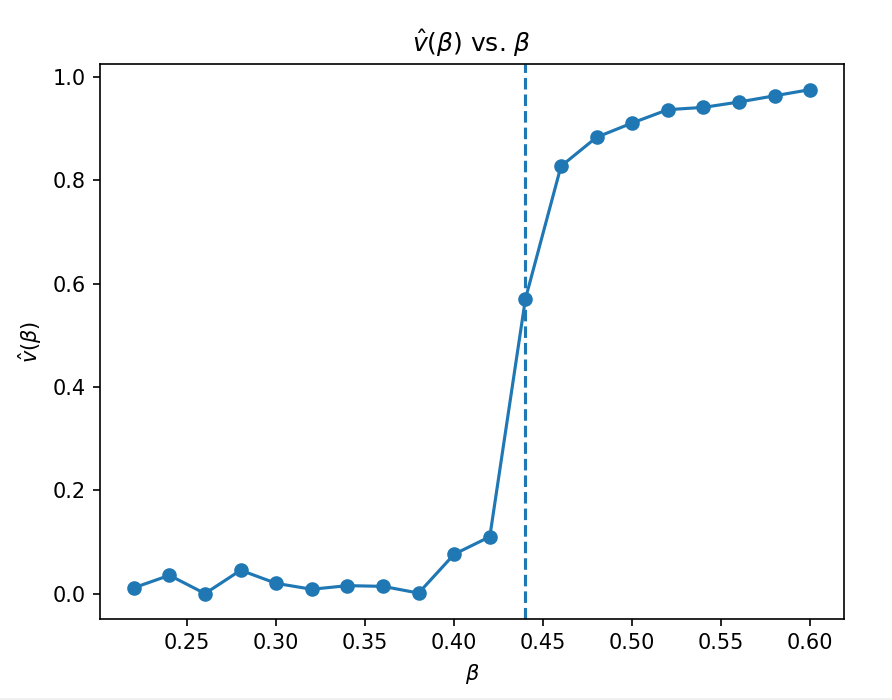
\includegraphics[width=0.6\textwidth]{Images/Estimator v Beta.png}
        \end{wrapfigure}
      
        \pagebreak
        
        Finally, here is the full Python implementation of the model, plots, and estimator:
        
        \begin{center}
            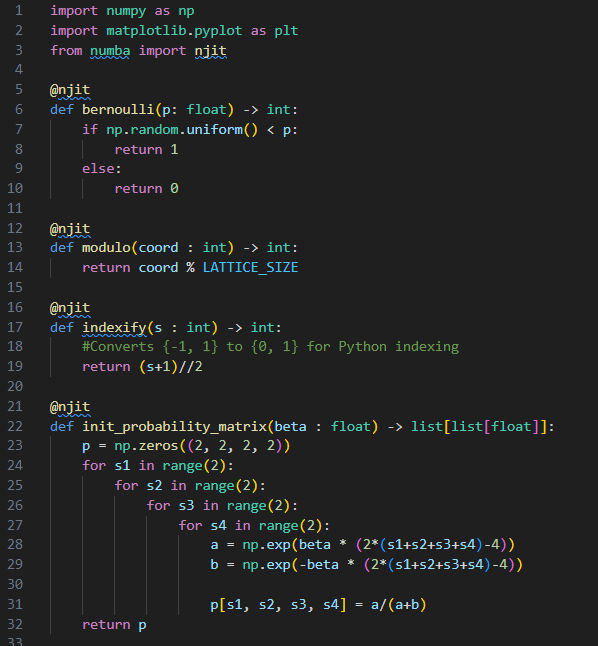
\includegraphics[width=\textwidth]{Images/Code 1 - Helper.png}
            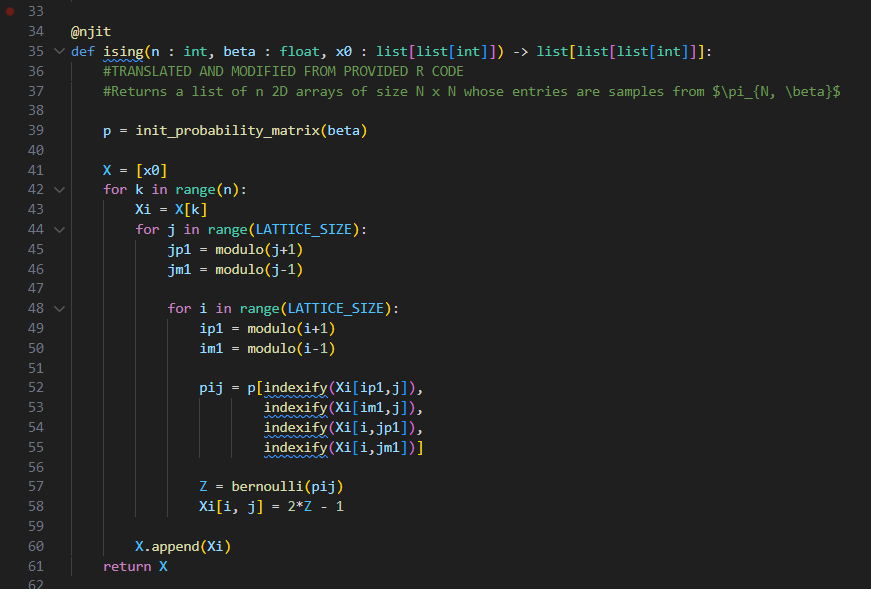
\includegraphics[width=\textwidth]{Images/Code 2 - Ising.png}
            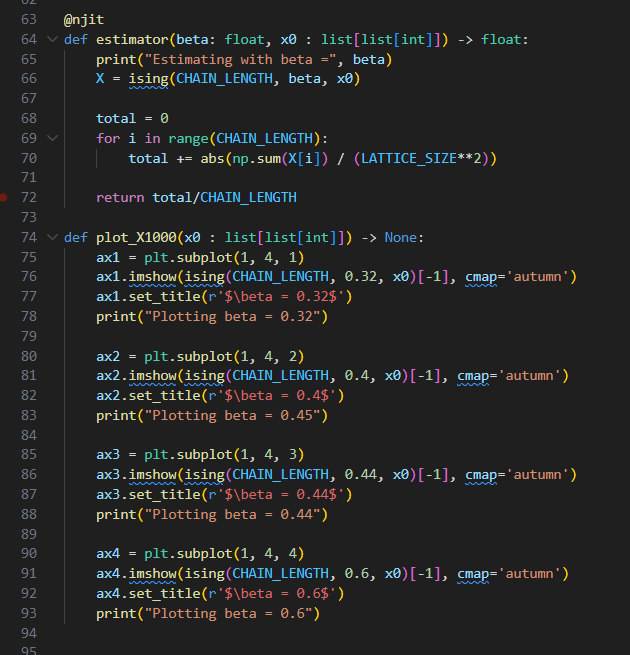
\includegraphics[width=\textwidth]{Images/Code 3 - Estimator.png}
            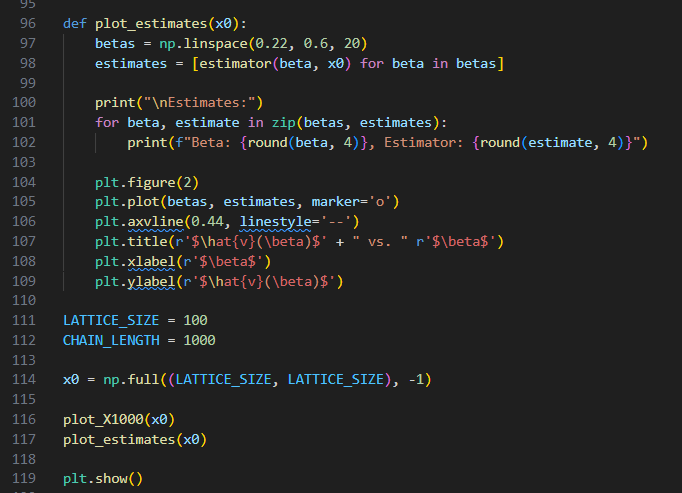
\includegraphics[width=\textwidth]{Images/Code 4 - Plotting.png}
        \end{center}
    \color{black}
%\bibliographystyle{plain}
\bibliography{sample}

\end{document}
